%% LyX 2.0.0 created this file.  For more info, see http://www.lyx.org/.
%% Do not edit unless you really know what you are doing.
\documentclass[10pt,a4paper,twoside,french]{article}
\usepackage[T1]{fontenc}
\usepackage[utf8]{inputenc}
\usepackage{babel}
\addto\extrasfrench{%
   \providecommand{\og}{\leavevmode\flqq~}
   \providecommand{\fg}{\ifdim\lastskip>\z@\unskip\fi~\frqq}
}

\usepackage{float}
\usepackage{graphicx}
\usepackage[unicode=true,pdfusetitle,
 bookmarks=true,bookmarksnumbered=false,bookmarksopen=false,
 breaklinks=false,pdfborder={0 0 1},backref=section,colorlinks=false]
 {hyperref}
\usepackage{breakurl}

\makeatletter

%%%%%%%%%%%%%%%%%%%%%%%%%%%%%% LyX specific LaTeX commands.
\special{papersize=\the\paperwidth,\the\paperheight}


%%%%%%%%%%%%%%%%%%%%%%%%%%%%%% User specified LaTeX commands.
%% Exemple de source LaTeX pour un article soumis à TALN




% Package utilisé uniquement pour l'exemple.
\usepackage{lipsum}

% faire les \usepackage dont vous avez besoin AVANT le \usepackage{jeptaln2012} 
% add the \usepackage for you packages BEFORE the \usepackage{jeptaln2012}

\usepackage{jeptaln2012}% Insérer les définitions de biblio en français (cf apalike-fr.bst)

\makeatother

\begin{document}

\title{Détection de transcriptions incorrectes de parole non-native dans
le cadre de l’apprentissage de langues étrangères}


\author{Luiza Orosanu\quad{}Denis Jouvet\quad{}Dominique Fohr\quad{}Irina
Illina\quad{}Anne Bonneau \\
 {\small INRIA - LORIA, 615 rue de Jardin Botanique 54600 Villers-les-Nancy}\\
{\small{} }\texttt{\small{} \{luiza.orosanu, denis.jouvet, dominique.fohr,
irina.illina, anne.bonneau\}@loria.fr }{\small{} }\\
{\small{} }}

\maketitle
\resume{ Cet article analyse la détection de transcriptions incorrectes
de parole non-native dans le contexte de l’apprentissage de langues
étrangères. L’objectif est de détecter et rejeter les transcriptions
incorrectes (i.e. celles pour lesquelles le texte ne correspond pas
au signal de parole associé) tout en étant tolérant aux défauts de
prononciation inhérents à la parole non-native. L’approche proposée
exploite la comparaison d’un alignement contraint par la transcription
à vérifier avec un alignement non contraint correspondant à un décodage
phonétique. Plusieurs critères de comparaison sont décrits et combinés
par l’intermédiaire d’une fonction de régression logistique. L'article
analyse l’influence de divers paramétrages comme l’impact des variantes
de prononciation non-natives, l’utilisation de fonctions de décision
spécifiques à la longueur des transcriptions, et l’impact d’un apprentissage
de la fonction de décision avec la parole native ou non-native. Les
évaluations de performances sont menées à la fois sur des corpus de
parole natives et non-natives. }

\abstract{Detection of incorrect transcriptions of non-native speech
in the context of foreign language learning }{This article analyses
the detection of incorrect transcriptions of non-native speech in
the context of foreign language learning. The purpose is to detect
and reject incorrect transcriptions (i.e. those for which the text
does not correspond to the associated speech signal) while being tolerant
to the pronunciation defects of non-native speech. The proposed approach
exploits the comparison between two alignements: one constrained by
the transcript which is being checked, with an other one unconstrained,
corresponding to a phonetic decoding. Several criteria are described
and combined via a logistic regression function. The article analyzes
the influence of different settings, such as the impact of non-native
pronunciation variants, the use of decision functions dependent on
the length of the transcriptions, and the impact of learning decision
functions on native or non-native speech. The performance evaluations
are conducted both on native speech and non-native speech. }

\motsClefs{Apprentissage d'une langue étrangère, entrées incorrectes,
parole non-native, variantes de prononciation, alignements contraint
et non-contraint} {Foreign language learning, incorrect transcriptions,
non-native speech, pronunciation variants, constrained and unconstrained
alignements}


\section{Introduction}

L’aide à l’apprentissage des langues étrangères est un domaine d’application
de la reconnaissance automatique de la parole qui s’est développé
ces dernières années. L’objectif est de détecter et signaler à l’apprenant
ses erreurs ou défauts de prononciation, afin qu’il puisse les corriger,
et peu à peu améliorer sa maîtrise de la langue étrangère. L’une des
principales difficultés pour ces systèmes est la détection et la localisation
automatique des défauts de prononciation \cite{Herron99automaticlocalization}
tout en restant robuste à la parole non-native. Des méthodes ont été
proposées pour déterminer un score de qualité de prononciation \cite{Witt200095}
en exploitant des rapports de vraisemblance. De tels systèmes tirent
profit de l’introduction de modèles acoustiques de phonèmes de la
langue maternelle (en complément des modèles des phonèmes de la langue
cible) ainsi que de la connaissance des défauts (variantes) possibles
de prononciation non-natives.

Un autre élément important de l’apprentissage des langues concerne
la prosodie. Certains projets ont porté sur le retour d’information
sur les erreurs de durée \cite{Eskenazi00thefluency} mais le retour
d’information prosodique se résume fréquemment à jouer ou rejouer
une prononciation du mot ou de la phrase par un locuteur natif. Une
méthode originale a été proposée dans \cite{foreignLanguage} qui
vise à améliorer simultanément la production et la perception en combinant
un retour prosodique précis et détaillé et un retour sonore basé sur
une modification prosodique de la prononciation de l’apprenant. Cette
approche nécessitant une segmentation phonétique de la prononciation
de l’apprenant, une étude de la pertinence de la segmentation phonétique
a été entreprise \cite{MESBAHI_Reliability}. Ces méthodes automatiques
de diagnostic des prononciations reposent sur une segmentation phonétique
du signal de parole qui est obtenue par alignement forcé du signal
de parole avec les modèles correspondant à la phrase prononcée. La
prise en compte de variantes de prononciation non natives améliore
la qualité des alignements \cite{nonNative}. 

Cependant, il arrive que le signal acoustique ne corresponde pas à
la phrase attendue (erreur de prononciation, parole parasites, problème
de capture du son, …). Le système doit donc être capable de déterminer
si le signal audio correspond ou pas à la phrase attendue. Ce type
de décision correspond typiquement au rejet des entrées incorrectes
ou des mots hors vocabulaire en reconnaissance de la parole \cite{outOfVocabulary,boite2000traitement}.
Contrairement à ces approches, qui visent essentiellement la parole
native, ici nous voulons offrir un soutien à l'apprentissage des langues
étrangères, et donc nous avons besoin de détecter les incohérences
(i.e. un signal audio ne correspondant pas à la phrase attendue),
mais en même temps tolérer les défauts de prononciations non-natives.

Donc, l'objectif de cet article est d'étudier en détail le rejet de
transcriptions incorrectes dans le contexte de l'apprentissage des
langues étrangères. La première partie présente une description de
la méthodologie mise en œuvre, et en particulier les critères utilisés
et la fonction de décision choisie. La deuxième partie du papier est
consacrée à la description des expériences menées et à la discussion
des résultats.


\section{Méthodologie\label{sec:Methodologie}}

Afin de rejeter les transcriptions incorrectes, tout en acceptant
celles qui sont correctes, il faut déterminer si le signal audio et
la transcription correspondent. Pour cela, nous avons choisi de décoder
les signaux audio de deux façons différentes. Tout d'abord, nous effectuons
un décodage contraint, où l'on force le système à suivre la séquence
des mots présents dans la transcription de référence. Ensuite, nous
effectuons un décodage non-contraint, où l'on donne au système la
liberté de choisir n’importe quel phonème pour n’importe quelle position
dans la phrase. Finalement, nous comparons les deux alignements (contraint
et non-contraint) afin de décider si la transcription est correcte
ou non (i.e. si elle correspond ou pas au signal audio).


\subsection{Critères pour la décision\label{sub:Criteres}}

Cette partie décrit les critères choisis pour différencier les transcriptions
correctes de celles qui sont incorrectes. Ces critères sont basés
sur des informations provenant des alignements contraints et non-contraints,
en considérant les phonèmes, les trames ou les zones annotées silence/bruit. 

\textbf{1. Critère associé aux phonèmes: }pourcentage de segments
phonétiques qui ont le même label dans les deux alignements et dont
au moins une limite temporelle diffère de moins de 20 ms. Les segments
de silence/bruit sont ignorés. Sa valeur est bien plus grande pour
les transcriptions correctes que pour celles incorrectes. 
\begin{figure}[H]
\centering{}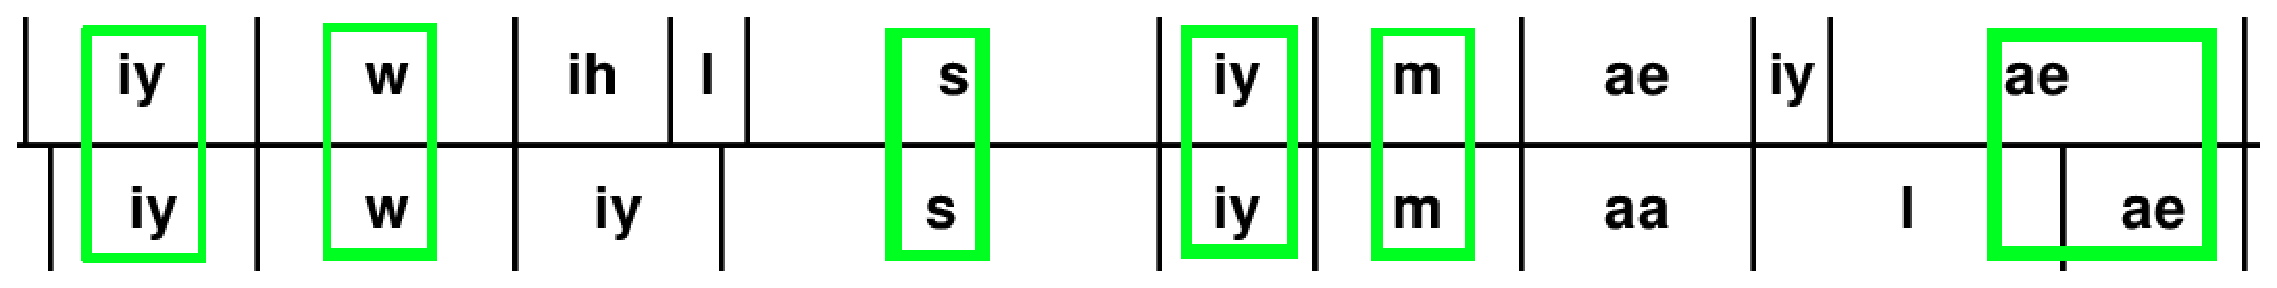
\includegraphics[scale=0.24]{Image/ph}

\caption{Exemple de transcription correcte avec ses deux décodages: contraint
(en haut) et non-contraint (en bas). Les rectangles verts indiquent
les phonèmes pris en compte pour calculer le <<critère associé aux
phonèmes >> }
\end{figure}


\textbf{2. Critère associé aux trames: }basé sur l'étiquetage des
trames. Même si le décodage phonétique ne trouve pas le bon phonème,
il est susceptible de le remplacer avec un phonème de la même classe.
Une classe phonétique est représentée par des sons qui partagent au
moins une caractéristique phonétique, et en particulier le «mode d'articulation\textquotedbl{}.
Nous calculons alors le pourcentage de trames ayant leurs étiquettes
appartenant à la même classe phonétique. Ce pourcentage est donc généralement
plus grand pour les transcriptions correctes que pour celles incorrectes.
Dans l'exemple suivant nous avons considéré les classes phonétiques:
voyelles (V), semi-voyelles (SV), fricatives (F), nasales (N) et plosives
(P). 
\begin{figure}[H]
 \centering{}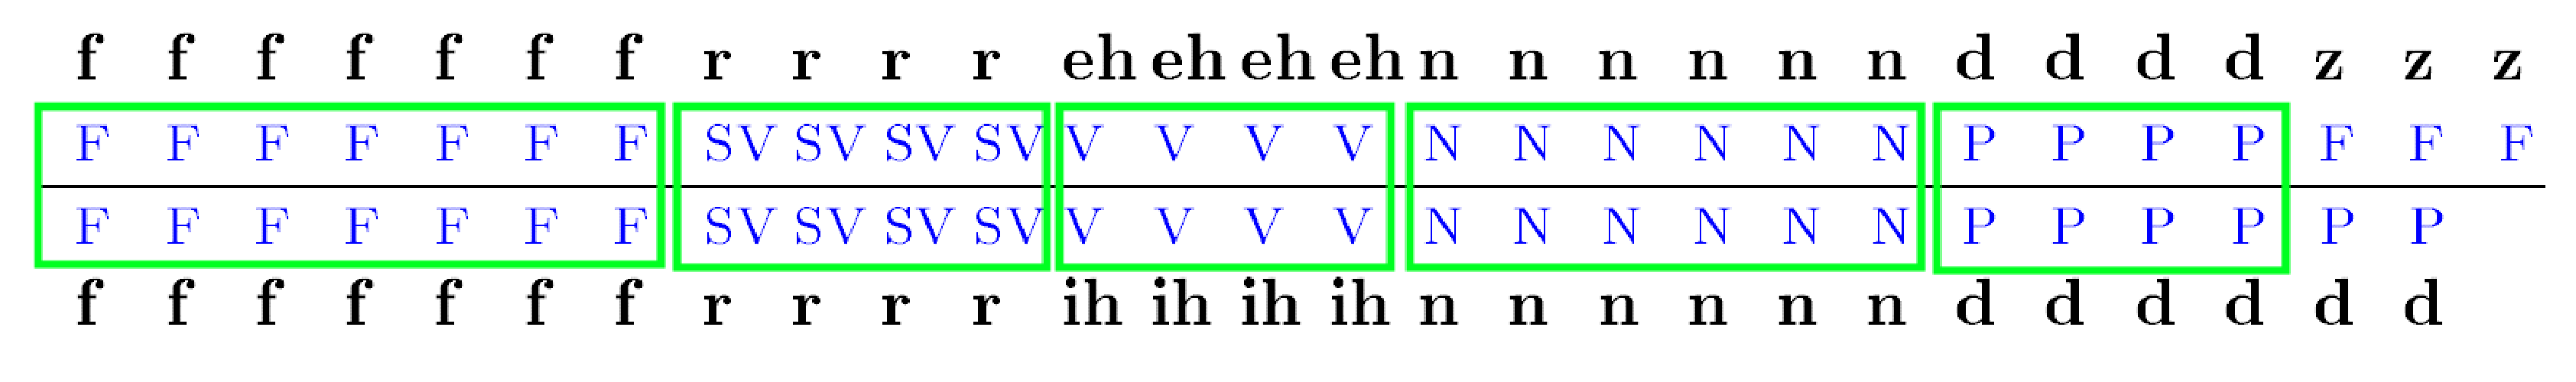
\includegraphics[scale=0.2]{Image/tr}\caption{Exemple de transcription correcte avec ses deux décodages: contraint
(en haut) et non-contraint (en bas). Les rectangles verts indiquent
les trames prises en compte pour calculer le <<critère associé aux
trames >> }
\end{figure}


\textbf{3. Critère associé aux zones de non-parole}: basé uniquement
sur les segments de non-parole (silence / bruit). Lorsque l'on force
le système à aligner un signal audio sur un texte qui ne lui correspond
pas (le cas d'une transcription incorrecte), il est fréquent que le
système ajoute plusieurs segments de silence entre les mots et/ou
qu'il augmente ou diminue la durée de ceux qui existent réellement.
Nous calculons donc la différence de recouvrement des segments de
non-parole entre les deux alignements (exprimée en pourcentage du
nombre total de trames). La valeur de ce critère sera plus petite
pour les transcriptions correctes que pour celles incorrectes. 
\begin{figure}[H]
 \centering{}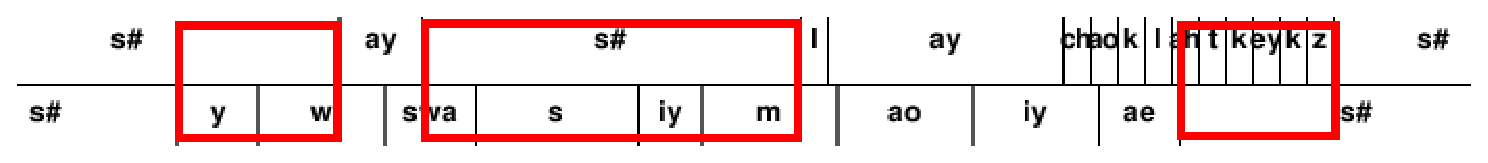
\includegraphics[scale=0.48]{Image/sil}\caption{Exemple de transcription incorrecte avec ses deux décodages: contraint
(en haut) et non-contraint (en bas). Les rectangles rouges indiquent
les trames prises en compte pour calculer le <<critère associé aux
zones de non-parole >> }
\end{figure}



\subsection{Classification de données}

Compte tenu des critères choisis pour la décision (section \ref{sub:Criteres})
et de la tâche de classification limitée à deux classes (\textit{correcte}
ou \textit{incorrecte}), le modèle prédictif de la régression logistique
\cite{Dreiseitl2002352} a été choisi comme classifieur binaire. En
général, la régression logistique est utilisée pour calculer la probabilité
d'appartenance à une classe parmi deux:\textbf{ 
\[
P\left(1|\overline{X},\alpha\right)=f(\overline{X})=\frac{1}{1+exp(-(\alpha_{0}+\alpha_{1}x_{1}+\alpha_{2}x_{2}+\alpha_{3}x_{3}))}
\]
 }

La première étape de l'approche consiste à apprendre les paramètres
du classifieur sur les données d'apprentissage. Le corpus d'apprentissage
est représenté par l'ensemble de données $D=\left\{ \overline{X_{i}},\: y_{i}\right\} ,\: i=1,...,N$
où: 
\begin{itemize}
\item $\overline{X}=<x_{1},x_{2},x_{3}>$ est le vecteur comprenant les
informations sur la transcription à classifier, c'est-à-dire les critères
par phonèmes, par trames et par zones de non-parole 
\item $y$ indique l’appartenance à la classe correcte ($y=1$) ou à la
classe incorrecte ($y=0$) 
\item $N$ est le nombre de transcriptions dans le corpus d'apprentissage. 
\end{itemize}
Les paramètres $\overline{\alpha}=<\alpha_{0},\alpha_{1},\alpha_{2},\alpha_{3}>$
sont déterminés par l'estimation du maximum de vraisemblance, qui
se calcule en minimisant la fonction d'erreur:

\begin{center}
\textbf{$E=-\sum_{i=1}^{N}\left(y_{i}\,\cdot\, ln\left(f(\overline{X_{i}})\right)\,+\,\left(1-y_{i}\right)\,\cdot\, ln\left(1-f(\overline{X_{i}})\right)\right)$} 
\par\end{center}

La minimisation est effectuée par la méthode de la descente du gradient.
Cet algorithme d'optimisation numérique vise à obtenir un optimum
(éventuellement local) par améliorations successives. A partir d'un
point de départ $\alpha$ et une valeur initiale du pas de descente,
les paramètres sont modifiés jusqu'à atteindre la condition d’arrêt
(plus d’amélioration possible).

Apres, les courbes DET (<<detection error tradeoff >>) sont utilisées
pour présenter les résultats obtenus sur les données de test . Une
courbe DET est un graphique des taux d'erreur pour les systèmes de
classification binaire. Elle est utilisée ici comme un moyen de représenter
les performances sur la tâche de classification des transcriptions,
qui implique un compromis entre les taux de <<\textit{fausse acceptation}
>> (\textit{FA}, le pourcentage de transcriptions incorrectes, mais
classées comme étant correctes par le système) et de <<\textit{faux
rejet} >> (\textit{FR}, le pourcentage de transcriptions correctes,
mais classées comme étant incorrectes par le système). Une transcription
est acceptée seulement si la valeur de la régression logistique \textbf{$f(\overline{X})$}
est supérieure à un seuil $\sigma$ . Pour tracer la courbe DET, différentes
valeurs du seuil $\sigma\epsilon[0,1]$ sont utilisées. Les taux d'erreurs
(FA, FR) pour chaque valeur du seuil sont indiqués sur le graphique.
Finalement, le meilleur compromis entre les taux d'erreur (parmi tous
les points disponibles sur les graphiques \textit{DET}), est celui
qui maximise la F-mesure: 
\begin{equation}
\frac{1}{F}=\frac{1}{2}\left(\frac{1}{1-FA}+\frac{1}{1-FR}\right)\label{eq:F-mesure}
\end{equation}



\section{Expériences et résultats}


\subsection{Contexte expérimental}

Afin d'évaluer les approches mentionnées dans la section \ref{sec:Methodologie},
deux corpus anglais de parole native et non-native sont utilisés.
Ils proviennent du projet INTONALE \cite{dargnatMth} consacré à l'étude
prosodique. Le corpus natif contient environ 1500 signaux audio qui
ont été enregistrés par 22 locuteurs (15 femmes et 7 hommes) anglais
(66 phrases par locuteur). Le corpus non-natif contient environ 800
signaux audio qui ont été enregistrés par 34 locuteurs (29 femmes
et 5 hommes) français (23 phrases par locuteur). Ces enregistrements
ont été faits dans une pièce calme. Le logiciel développé pour l’enregistrement
des mots ou des phrases affiche sur l’écran la phrase à prononcer.
Le locuteur peut ensuite choisir, après chaque prononciation d'une
phrase, de la répéter (en cas de problème) ou de passer à la suivante.

Les corpus utilisés contiennent tous des transcriptions correctes
(même si la parole non-native est sujette à beaucoup de défauts de
prononciation). Pour simuler des transcriptions incorrectes, nous
utilisons les mêmes signaux audio, mais nous attachons à chacun une
transcription qui ne lui correspond pas (tirée de façon aléatoire
parmi les autres). Nous avons donc la même quantité de données correctes
et incorrectes. 

Chaque corpus, natif ou non-natif, est découpé en deux parties égales:
une partie pour faire l’apprentissage des paramètres $\overline{\alpha}$,
et l'autre pour évaluer les performances. Afin d'étudier la dépendance
des paramètres à la longueur des transcriptions (nombre des phonèmes),
chaque corpus est de nouveau découpé en 3 sous-ensembles : transcriptions
courtes (moins de 19 phonèmes), transcriptions moyennes et transcriptions
longues (plus de 30 phonèmes).

Les outils HTK \cite{Young2002} sont utilisés pour le décodage des
signaux audio. Les modèles acoustiques ont été appris en utilisant
le corpus anglais TIMIT \cite{timit}. Ses signaux audio ont été enregistrés
par 630 locuteurs américains, avec une fréquence d'échantillonnage
de 16 kHz. L'analyse acoustique MFCC (Mel Frequency Cepstral Coefficients)
donne 12 paramètres MFCC et le logarithme de l'énergie par trame (fenêtre
de 32 ms, décalage de 10ms). La segmentation phonétique d'une transcription
(décodage contraint) est obtenue avec des modèles acoustiques HMM
(Hidden Markov Models) et la prise en compte des variantes de prononciation
de chaque mot. Chaque état d'un modèle HMM a été modélisé par un mélange
de 16 gaussiennes.

Deux lexiques ont été utilisés: le premier inclut seulement les variantes
natives pour chaque mot (lexique natif: \textit{CMU dictionary} \cite{cmu})
et le second inclut en plus des variantes non-natives (lexique non-natif).
Un grand nombre de variantes de prononciation non-natives observées
dans le corpus de parole non-native ont été incluses dans le lexique
de prononciation \cite{MESBAHI_Reliability} (la génération automatique
de variantes de prononciation non-natives sera étudiée dans les travaux
futurs).


\subsection{Évaluations \label{sub:Evaluations}}

Cette partie étudie l'impact de différents paramètres de l’approche,
en particulier pour le traitement de la parole non-native: l'impact
du lexique de prononciation natif ou avec variantes non-natives, l'impact
d'une fonction de décision globale, ou d'une fonction dépendante de
la longueur de la transcription traitée et l'impact du type des données
(natives ou non-natives) utilisées pour l'apprentissage des paramètres. 

\begin{figure}[H]
\centering{}\includegraphics[scale=0.38]{Image/jep1}\hspace{0.1cm}\includegraphics[scale=0.38]{Image/jep2}\caption{{\small Courbes DET pour les lexiques natif et non natif, et le paramétrage
global (courbes rouges / bleues) ou dépendant de la longueur des transcriptions
(courbes vertes / mauves) }}


\label{Fig:Sigmoid} 
\end{figure}


\begin{figure}[H]
\centering{}\includegraphics[clip,scale=0.38]{Image/jep3}\hspace{0.1cm}\includegraphics[scale=0.38]{Image/jep4}\caption{{\small Courbes DET pour l'apprentissage sur les corpus natif et non-natif,
et le lexique natif (courbes en jaune-vert / bleu-nuit) ou non-natif
(courbes en bleu-ciel / marron). Le paramétrage est dépendant de la
longueur des transcriptions.}}


\label{Fig:Lexique} 
\end{figure}


La Figure \ref{Fig:Sigmoid} montre que l'utilisation des fonctions
sigmoïdes dépendantes de la longueur des transcriptions, donne de
meilleures résultats que l'utilisation d'une fonction de décision
unique (globale), quel que soit le corpus utilisé et quel que soit
le lexique associé. 

La Figure \ref{Fig:Lexique} montre que l'utilisation d'un lexique
natif est nécessaire pour le corpus natif. Cependant, pour le corpus
non-natif, les deux lexiques donnent des résultats similaires. Les
résultats montrent également qu'il est important d'apprendre les fonctions
de décision sur les données non-natives pour obtenir des résultats
optimaux sur le corpus non-natif. En revanche, l'influence du corpus
d'apprentissage semble négligeable pour le traitement de la parole
native.

Les meilleurs résultats obtenus pour le corpus natif sont: un taux
de \textit{fausse acceptation} de 6.35\% avec un taux de \textit{faux
rejet} de 9.53\%, qui correspondent à une \textit{F} mesure (eq. \ref{eq:F-mesure})
de 92.031\%.

Les meilleurs résultats obtenus pour le corpus non-natif sont: un
taux de \textit{fausse acceptation} de 4.88\% avec un taux de \textit{faux
rejet} de 6.68\% (qui correspondent à une F mesure de 94.207\%). Par
comparaison, lorsque la décision (acceptation/rejet) est effectuée
en considérant un seul critère à la fois, nous obtenons pour le critère
associé aux phonèmes, F=88.686\%, pour celui associé aux trames, F=86.986\%
et, pour celui associé aux zones de non-parole, F=78.563\%.


\section{Conclusions}

Cet article a étudié le rejet des transcriptions incorrectes de parole
non-native dans le cadre de l’apprentissage d’une langue étrangère.
Quelques questions se sont alors posées. Comment rejeter les entrées
incorrectes tout en tolérant les défauts de prononciations non-natives?
Quels méthodes et critères choisir afin de pouvoir différencier les
entrées correctes de celles incorrectes? L’exploitation de variantes
non-natives dans le lexique est-elle bénéfique? Les fonctions de décision
doivent-elles être spécifiques à la longueur des transcriptions? Sur
quel type de corpus (natif ou non-natif) doit-on faire l’apprentissage
de paramètres?

Pour répondre à toutes ces questions, nous avons utilisé deux corpus
anglais, l’un prononcé par des locuteurs natifs et l’autre par des
non-natifs. De plus, chaque corpus a été découpé en deux, une moitié
pour l’apprentissage et l’autre moitié pour les évaluations de performance.
Pour l’apprentissage des fonctions de décision dépendantes de la longueur
des transcriptions, trois catégories ont été considérées : transcriptions
courtes, moyennes et longues. Pour distinguer les transcriptions correctes
de celles incorrectes, nous comparons l’alignement contraint par la
transcription à vérifier avec l’alignement résultant d’un décodage
phonétique non-contraint. Cette comparaison a été faite en exploitant
trois critères calculés au niveau de phonèmes, de trames et de zones
de non-parole. Ces trois descripteurs sont combinés par une fonction
de régression logistique pour fournir la fonction de décision.

Les évaluations effectuées sur ces corpus montrent que: 
\begin{itemize}
\item l’utilisation de plusieurs fonctions de décision (sigmoïdes) dépendantes
de la longueur des transcriptions est plus performante que l’utilisation
d’une seule indépendante de la longueur des transcriptions. 
\item il est important d’apprendre les fonctions de décision sur des données
non-natives, en particulier pour le traitement de la parole non-native. 
\item l’utilisation de variantes de prononciation non-natives dans le lexique
des prononciations n’est pas nécessaire pour la tâche de vérification
des transcriptions, et même pénalisante si l’on traite de la parole
native. 
\end{itemize}
Le paramétrage optimal amène à des taux de fausse acceptation et faux
rejet raisonnables (4.88\% et 6.68\% pour le corpus de parole non-native).


\section*{Remerciements}

Les travaux présentés dans cet article font partie du projet ALLEGRO
(http://www.allegro-project.eu/), financé par le programme européen
INTERREG IV (http://www.interreg-fwvl.eu/fr/index.php).\bibliographystyle{apalike-fr}
\phantomsection\addcontentsline{toc}{section}{\refname}\bibliography{biblio}

\end{document}
